



\documentclass{article}
\usepackage[utf8]{inputenc}
\usepackage{graphicx}
\usepackage{hyperref}
\def\bibsection{\section*{References}}
%
\newcommand*{\fbinv}{\ensuremath{{\rm fb^{-1}}}\xspace}
\newcommand*{\pbinv}{\ensuremath{{\rm pb^{-1}}}\xspace}


\title{WG1 HL-LHC and HE-LHC Executive Summaries}
\author{Patrizia Azzi, Dieter Zeppenfeld, Stephen Farry, Paolo Nason, Alessandro Tricoli }
\date{November 2018}

\begin{document}

\maketitle

%%%%%%%%%%%%%%%%%%%%%%%%%%%%%%%%%%%%%
\section{HL-LHC Executive Summary}
%%%%%%%%%%%%%%%%%%%%%%%%%%%%%%%%%%%%%


%%%%%%%%%%%%%%%%
\subsection{QCD}

Studies of jet production at HL-LHC with $\sqrt{s}$ = 27 TeV $pp$ collisions and 3 ${\rm ab^{-1}}$ luminosity show that the uncertainty on the experimental jet energy scale can be reduced to a $2.5-5\%$ level in the range of the jet transverse momentum $p_T$ of 100 GeV $-$ 3 TeV, i.e. a factor 2 improvement on experimental precision with respect to Run-2 data, and that in inclusive jet and di-jet production measurements a $p_T$ of 5 TeV and an invariant mass ($m_{jj}$) of 9 TeV can be reached. Similar studies for inclusive isolated-photon production and isolated-photon with associated jet production show an extension of the kinematic reach up to 3.5 TeV in the photon $E_T$ and jet $p_T$, and up to 5 TeV in the photon-jet invariant mass $m_{\gamma - jet}$. Measurements of jet and photon production at the HL-LHC will allow to probe QCD perturbation theory at unprecedented energy scales with unprecedented precision as well as search for new physics in a new energy regime. 

\\
\\

Studies are carried out for the constraints on the quark and gluon structure of the proton expected from HL-LHC measurements in a range of physical
processes, from weak gauge boson and jet production to top quark and photon production. It is found that, in the invariant mass region $M_X > 100$ GeV, the HL-LHC measurements can be
expected to reduce the PDF uncertainties in processes such as Higgs boson or SUSY particle production
by a factor between 2 and 4, depending on the dominant partonic luminosity and on the scenario for the
systematic errors. Therefore, the exploitation of the HL-LHC constraints
on PDFs will feed into improved theoretical predictions for a range of phenomenologically relevant processes both within and beyond the SM. Figure~\ref{Fig:HLLHC_kin} shows the impact of HL-LHC data on the cross-section for gluino and quark-gluino production. 

\begin{figure}
\centering
%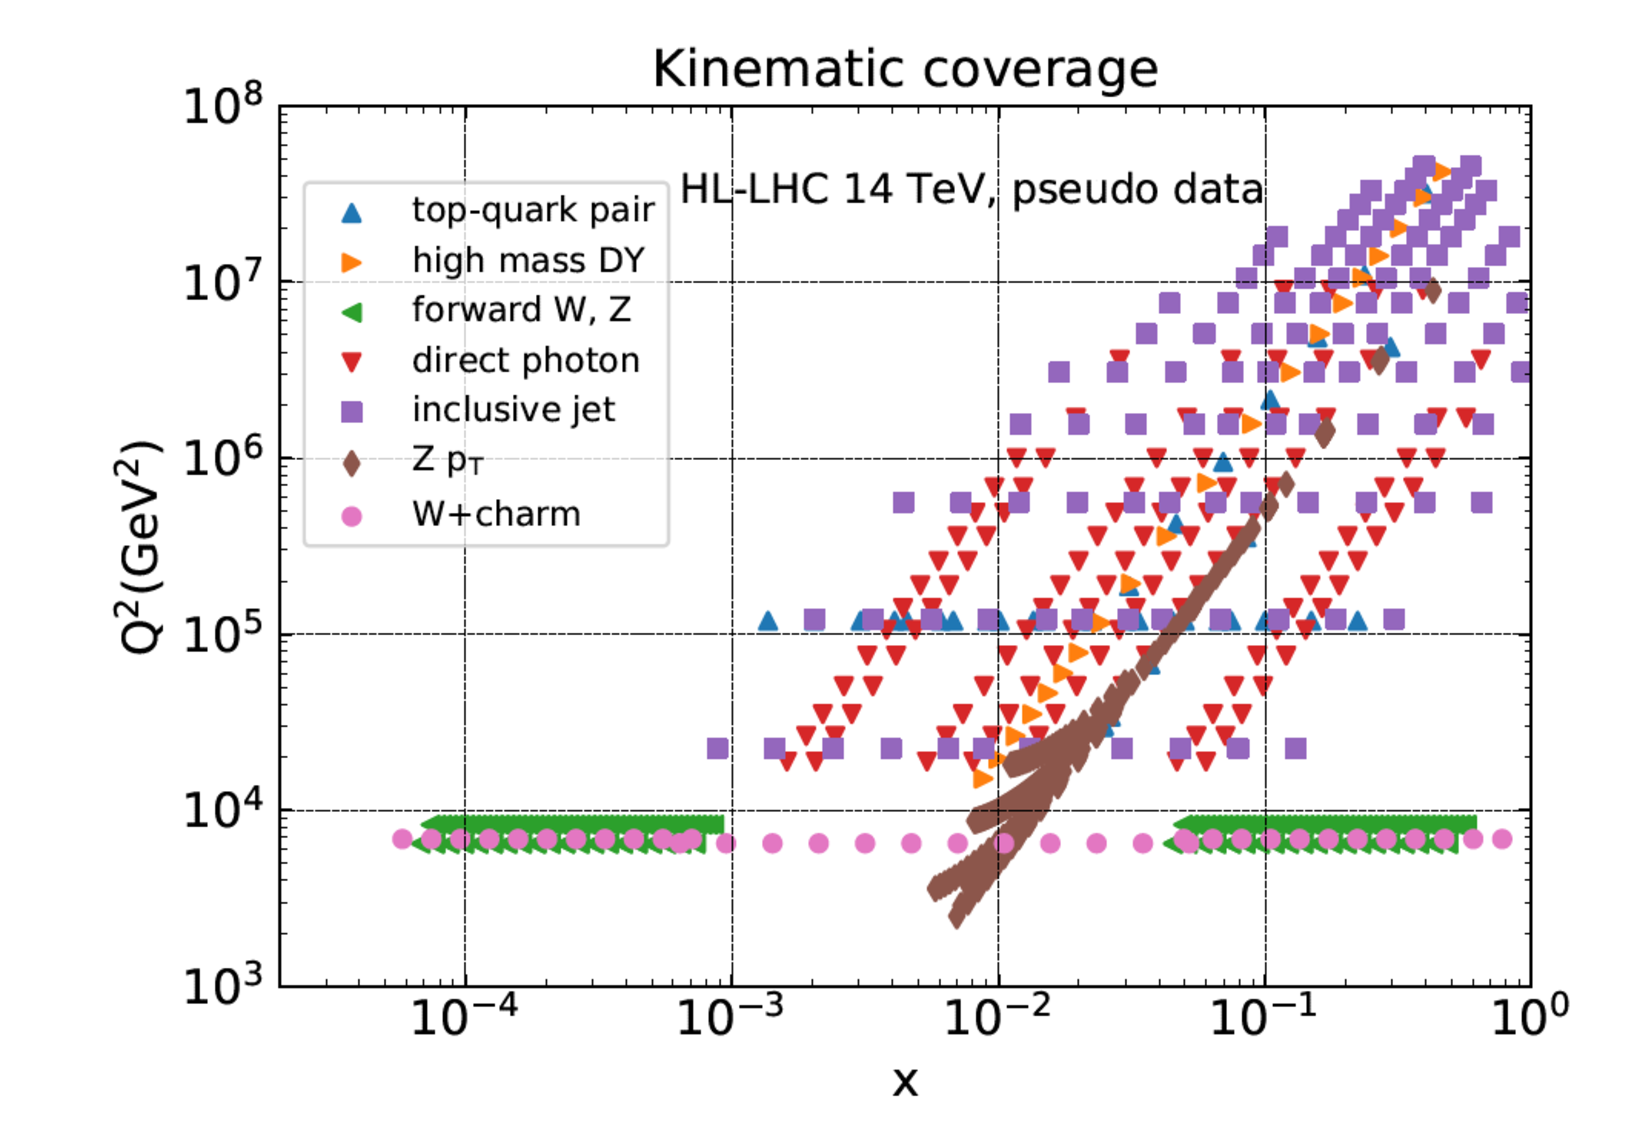
\includegraphics[width=0.7\textwidth]{HLLHC_kinematics.pdf}
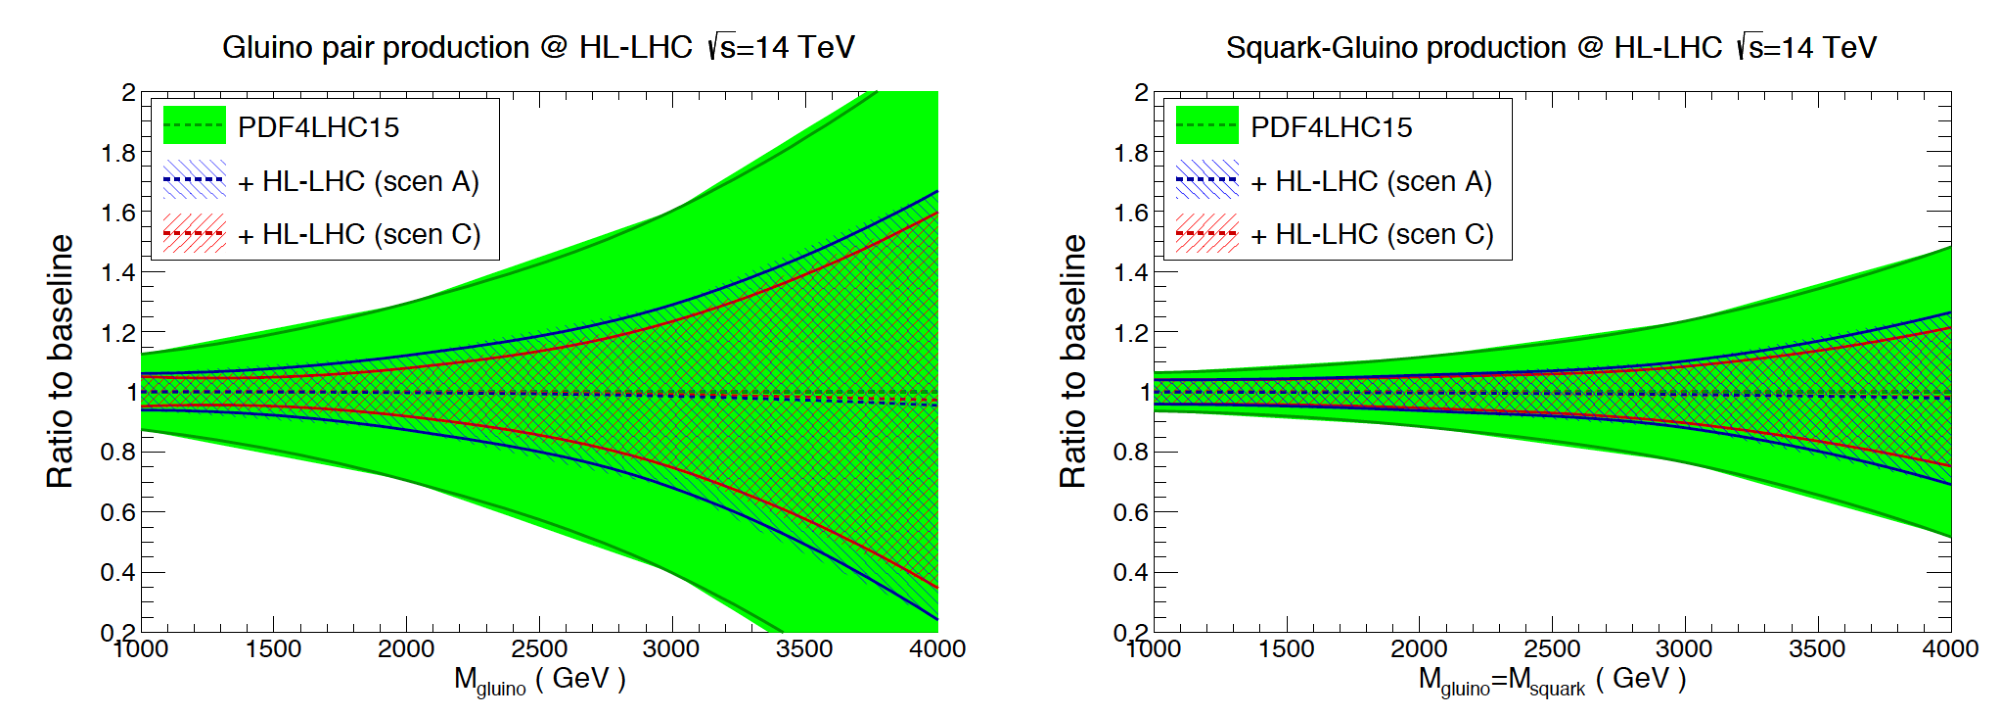
\includegraphics[width=1.0\textwidth]{UltimatePDF_gluino_squark.pdf}
%\caption{\label{Fig:HLLHC_kin} (Top) The kinematic coverage in the (x-${\rm Q^2}$) plane of HL-LHC pseudo-data. (Bottom) The cross sections for high-mass supersymmetric particle production at $\sqrt{s}$ = 14 TeV, comparing the predictions of the PDF4LHC15 baseline with those of the HL-LHC PDF sets in the conservative (A) and optimistic (C) scenarios, normalised to the central value of PDF4LHC15. The results corresponding to gluino pair production (left) and squark-gluino production (right). Ref.~\cite{Khalek:2018mdn}}
\caption{\label{Fig:HLLHC_kin} The cross sections for high-mass supersymmetric particle production at $\sqrt{s}$ = 14 TeV, comparing the predictions of the PDF4LHC15 baseline with those of the HL-LHC PDF sets in the conservative (A) and optimistic (C) scenarios, normalised to the central value of PDF4LHC15. The results corresponding to gluino pair production (left) and squark-gluino production (right). Ref.~\cite{Khalek:2018mdn}}
\end{figure}

\\
\\
The HL-LHC offers the opportunity to measure the effects of correlations between partons, via measurements of double-parton scattering (DPS) processes, for the first time. In same-sign WW production a good
observable to probe correlations is the lepton pseudorapidity asymmetry, which can only be nonzero in the presence of correlations. Theoretical calculations indicate values of the asymmetry at LHC energies on the
order of a few per cent, which should be measurable at the HL-LHC. By combining measurements of various processes sensitive to DPS at the HL-LHC we will ultimately be able to build up a picture of the correlations existing between partons in the proton.

%%%%%%%%%%%%%%%%
\subsection{EW}

{\bf Fig. : summary plot of experimental cross section precision for several VBS processes, combining results from ATLAS and CMS (ZZ, SS-WW, WZ, Tribosons, semilept WV). For Tribosons we also highlight the expected significance. One bin per analysis with current and projected precisions.}


\begin{table}[htbp]
\caption{Expected yields, cross sections and significances for electroweak processes at 14 TeV $pp$ collisions with 3000~ \fbinv of integrated luminosity.}
\label{tab:yields}
\begin{center}
\begin{tabular}{ | l | c | C | c| c|}
\hline
Process & Yield & $\sigma$ ${\rm [fb^{-1}]}$ & Significance & Precision {\rm $[\%]$} \\
\hline
\hline
$W^\pm W^\pm$ + jj $\to \ell^{\pm}\nu  \ell^{\pm}\nu$ + jj & .... & .... & ... & ...  \\
\hline
$ZZ$ + jj $\to \ell^{\pm}\ell^{\pm}  \ell^{\pm}\ell^{\pm}$ + jj & .... & .... & ...& ...    \\
\hline
$W^\pm Z$ + jj $\to \ell^{\pm}\nu  \ell^{\pm}\ell^{\pm}$ + jj & .... & .... & ...& ...    \\
\hline
$W^\pm V$ + jj $\to \ell^{\pm}\nu$ + jjjj & .... & .... & ... & ...   \\
\hline
\hline 
$W^{\pm} W^{\pm} W^{\mp} \to \ell^{\pm}\nu \ell^{\pm}\nu\ell^{\mp}\nu$ & .... & .... & ... & ...   \\
\hline 
$W^{\pm} W^{\pm} W^{\mp} \to \ell^{\pm}\nu \ell^{\pm}\nu jj$ & .... & .... & ... & ...   \\
\hline
$W^{\pm} W^{\mp} Z \to \ell^{\pm}\nu \ell^{\pm}\nu \ell^+\ell^-$ & .... & .... & ... & ...   \\
\hline 
$W^{\pm} W^{\mp} Z \to \ell^{\pm}\nu jj \ell^+\ell^-$ & .... & .... & ... & ...   \\
\hline
$W^{\pm} Z Z \to \ell^{\pm}\nu \ell^{+}\ell^{-} \ell^{+}\ell^{-}$ & .... & .... & ... & ...   \\
\hline
$W^{\pm} Z Z \to \ell^{\pm}\nu \ell^{+}\ell^{-} \nu\nu$ & .... & .... & ... & ...   \\
\hline 
$W^{\pm} Z Z \to \ell^{\pm}\nu  \ell^{+}\ell^{-} jj$ & .... & .... & ... & ...   \\
\hline 
$W^{\pm} Z Z \to jj \ell^{+}\ell^{-}  \ell^{+}\ell^{-} $ & .... & .... & ... & ...   \\
\hline
\end{tabular}
\end{center}
\end{table}



\\

The current world average of the weak mixing angle $\sin^2\theta_{eff}~=~0.23153~\pm~0.00016$ is dominated by the combination of measurements at LEP and at SLD, however, these two measurements differ by over 3 standard deviations. It will be of great scientific interest the study of the weak mixing angle at the HL-LHC: precision measurements may give insight into the tension between the previous measurements or may show signs of new physics. The measurement of $\sin^2\theta_{eff}$ at HL-LHC can reach a precision of $\pm~ 18 \cdot 10^{-5} ~= ~\pm 16 \cdot 10^{-5} ~({\rm PDF}) ~\pm~ 9 \cdot 10^{-5} ~({\rm exp.})$. The uncertainty will remain dominated by the currently limited knowledge of the PDFs. Considering the PDF-sensitive measurements at the HL-LHC using pseudo-data in prospect PDF fits the expected sensitivity of the
$\sin^2\theta_{eff}$ measurement with 3000~\ifb at
$\sqrt{s}$=14 TeV can be improved by $10\% - 25\%$ depending on the PDFs scenario considered.
Finally the sensitivity of the analysis to $\sin^2\theta_{eff}$ extraction is also estimated with a prospect PDF set including expected data from LHeC collider. In this case the PDF uncertainty is reduced by an additional factor of 5 with respect to the one obtained with the HL-LHC prospect PDFs.

\\

Proton-proton collision data are of great interest for $W$ boson physics. The $W$ production cross section is large enough to achieve small statistical uncertainties in a moderate run time at a low number of collisions per bunch crossing, pileup ($<\mu>$). At $\sqrt{s}$ = 14 TeV and for an instantaneous luminosity of $L\approx 5\cdot 10^{32} {\rm cm^{-2}s^{-1}}$, corresponding to $<\mu>$ = 2, about $2\cdot 10^{6}$ $W$ boson production events can be collected in one week, corresponding to a sample of 200 ${\rm pb^{-1}}$. Such a sample provides a statistical sensitivity at the permille level for cross section measurements, at the percent level for measurements of the $W$ boson transverse momentum distribution, and of about 10 MeV for a measurement of $m_W$. If five to ten weeks can be spent collecting such data in the course of the HL-LHC, a statistical precision of about 3 MeV can be reached. Given the importance of an optimal reconstruction of missing transverse momentum in this channel, low-pile-up runs are an important tool for precision measurements of the W boson properties.  Experimental systematic uncertainties are largely of statistical nature, and with adequate efforts and exploiting the full available data sample, their impact can be maintained at a level similar to the statistical uncertainty. The impact of PDF uncertainties on the $m_W$ measurement can be reduced to about 5–8 MeV, for a range of current PDF sets, when exploiting the extended coverage allowed by detectors at the HL-LHC. These uncertainties are further reduced to about 4 MeV when using the anticipated HL-LHC PDF set.
If the LHeC is built and runs synchronously with the HL-LHC, the combination of the large acceptance and excellent performance of the upgraded detectors and of the additional constraints on the proton structure from the theoretically clean DIS data reduces PDF uncertainties to less than 2 MeV. Figure ~\ref{Fig:Wmass} shows the expected precision on the $m_W$ measurement at the HL-LHC with $<\mu>$ = 2, for 200 ${\rm pb^{-1}}$ and 1 ${\rm fb^{-1}}$ of integrated luminosities, under different PDF scenarios from current PDF sets to the expected ultimate HL-LHC PDF set and with LHeC constraints.

\begin{figure}
\centering
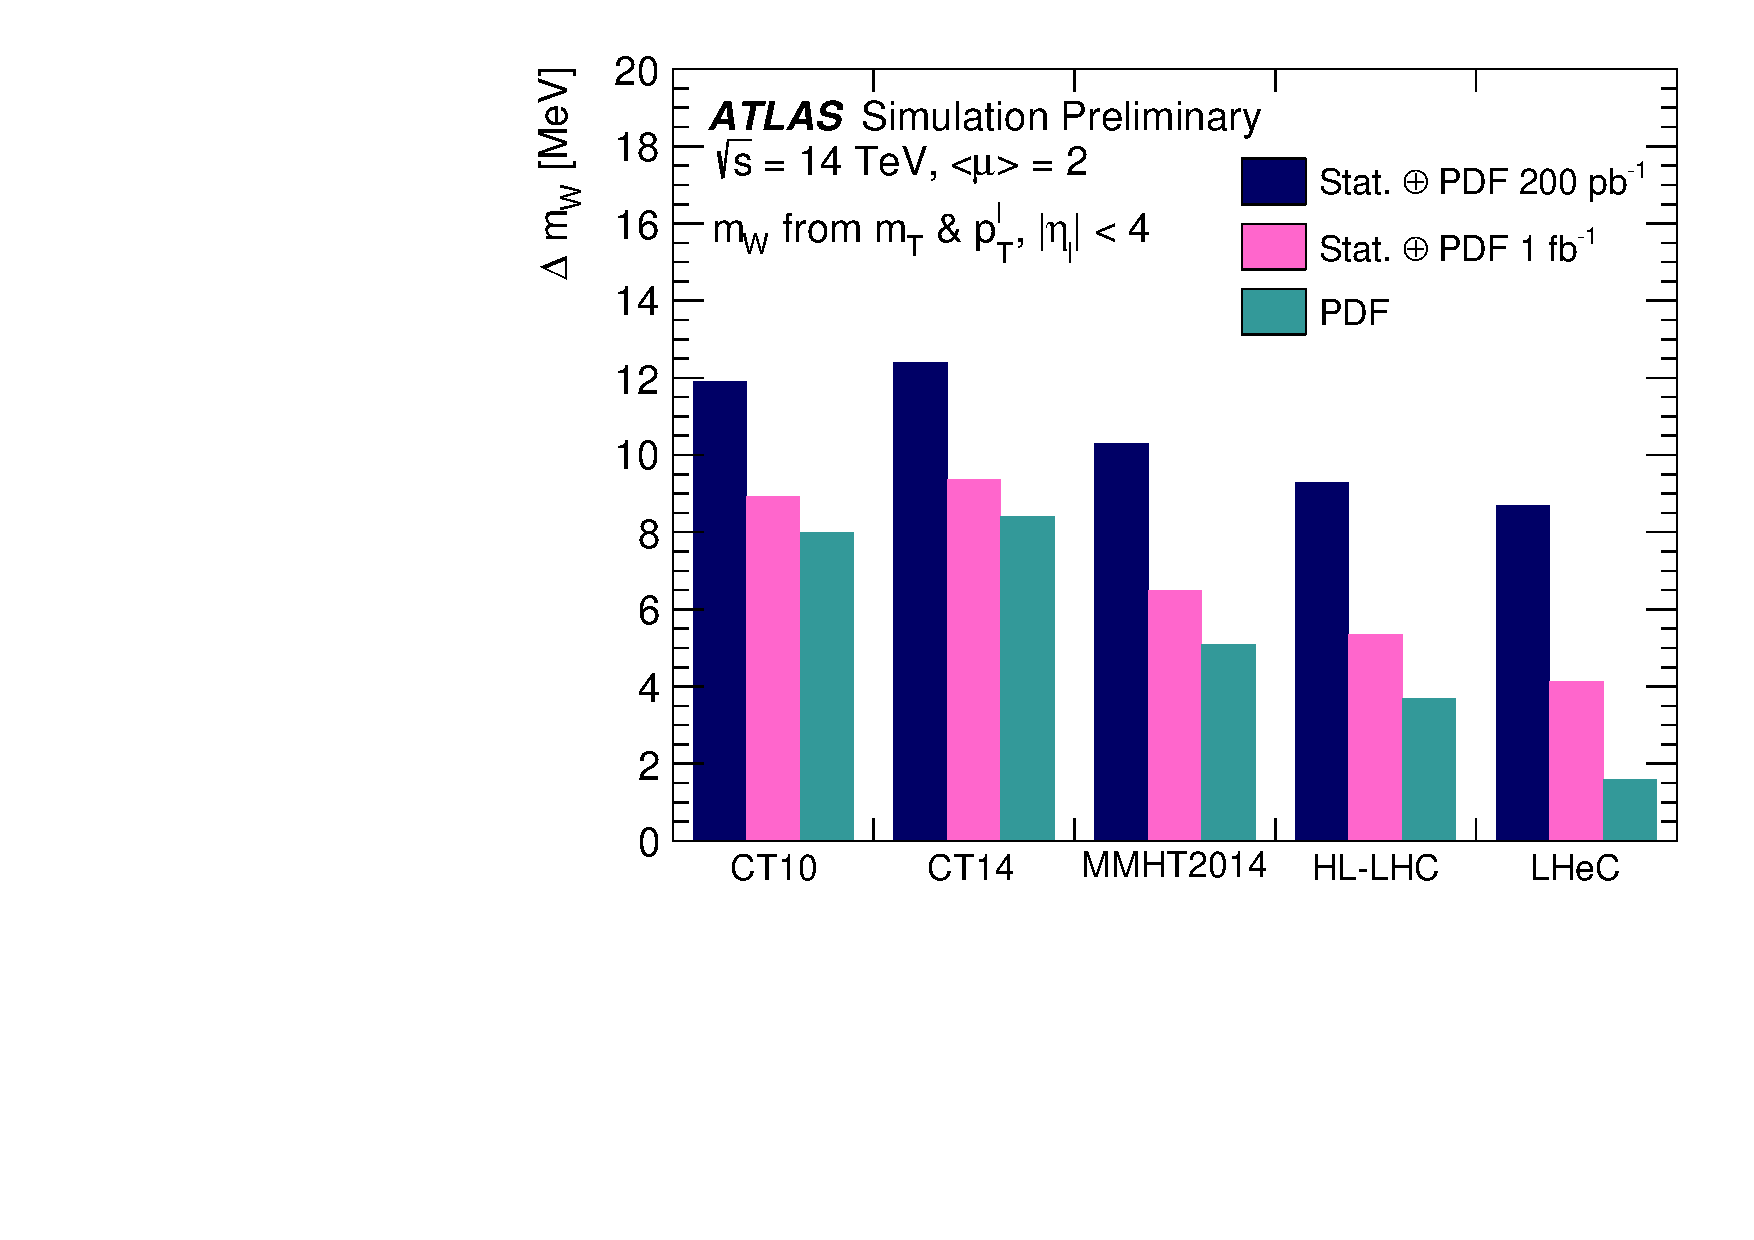
\includegraphics[width=0.9\textwidth]{Wmass_fig_06.pdf}
\caption{\label{Fig:Wmass} The expected statistical and PDF uncertainties on the $W$ mass measurement for different PDF sets, inclusing CT10, CT10, MMHT2014 as well as the predicted Ultimate PDF (HL-LHC) and LHeC PDF,  for the cases of 200 ~\pbinv ~and 1 ~\fbinv~  integrated luminosities, collected at ${\rm \sqrt{s}=14}$ TeV $pp$ collisions at the HL-LHC.}
\end{figure}


%%%%%%%%%%%%%%%%
\subsection{Forward/soft Physics}

{\bf Text: forward electroweak processes, i.e. gamma-induced processes, and reach in EFT limit setting}

%%%%%%%%%%%%%%%%
\subsection{Top}


{\bf Fig. on top mass, combining ATLAS and CMS, for example one bin per method with current and projected errors}


\\
{\bf Fig.: summary of precisions (when necessary significance) of several top process cross section measurements (e.g.4-tops, diff. Xsect tt and single top). One bin per analysis with current and projected precisions.}


\\
{\bf Textual discussion on top physics reach in precision (e.g. differential cross sections) and rare processes}


\\
{\bf Text: FCNC reach compared to current limits (to be shared with other WG's)}

%%%%%%%%%%%%%%%%
\subsection{All}


{\bf Fig.: summary of EFT improvements wrt current limits from Top and EW processes (and Higgs) - to be shared with Higgs group}


\\
{\bf Table: summary of EW fits highlighting increased precision, one row per observable, one column of current and one column for projected precisions}



\clearpage
%%%%%%%%%%%%%%%%%%%%%%%%%%%%%%%%%%%%%
\section{HE-LHC Executive Summary}
%%%%%%%%%%%%%%%%%%%%%%%%%%%%%%%%%%%%%

%%%%%%%%%%%%%%%%
\subsection{QCD}

Study of prospects for jet and di-jet production measurements show that at HE-LHC with $\sqrt{s}$ = 27 TeV $pp$ collisions and $15~ {\rm ab^{-1}}$ luminosity the kinematic reach can be extended up to 9 TeV in the jet transverse momentum $p_T$ and up 15 TeV in the di-jet invariant mass $m_{jj}$. It corresponds to a 4 TeV and 6 TeV extension of the HL-LHC reach with $3~ {\rm ab^{-1}}$, respectively in $p_T$ and $m_{jj}$. Similarly, studies of inclusive isolated-photon production and isolated-photon with associated jet production show an extension of the kinematic reach up to 5 TeV in the photon $E_T$ and jet $p_T$, and up to 12 TeV in the photon-jet invariant mass $m_{\gamma - jet}$. It corresponds to an extension of the HL-LHC reach in the photon $E_T$ and jet $p_T$ of 1.5 TeV, and of 7 TeV in $m_{\gamma - jet}$ with $3 ~{\rm ab^{-1}}{\rm ab^{-1}}$ luminosity.
The considerable increase in kinematic reach in jets and photons will allow to probe QCD perturbation theory, constrain PDF and search for new physics at unprecedented energy scales at the HE-LHC.
%%%%%%%%%%%%%%%%
\subsection{EW}

{\bf Table: summary of cross sections at 14 and 27 TeV, one row for 14 TeV one row for 27 TeV and one column per process (or above a kin. cut) }



\\
{\bf Fig.: reach in semilept WV, and aQGC limits wrt HL-LHC}



%%%%%%%%%%%%%%%%
\subsection{Top}

{\bf Table: summary of top cross sections at 14 and 27 TeV, one row for 14 TeV one row for 27 TeV and one column per process (or above a kin. cut) }



\\
{\bf Fig.: FCNC reach compared to HL (shared with other WG's)}


%%%%%%%%%%%%%%%%
\subsection{All}

{\bf Fig.: summary plot of EFT improvements wrt HL limits}

%%%%%%%%%%%%%%%%%%%%%%%%%%%%%%%%%%%%
\bibliographystyle{elsarticle-num}
\bibliography{references}{}
%%%%%%%%%%%%%%%%%%%%%%%%%%%%%%%%%%%%
\end{document}
%%%%%%%%%%%%%%%%%%%%%%%%%%%%%%%%%%%%
